\documentclass[12pt]{article}
\usepackage{graphicx,amsmath}
\usepackage{epsfig}

\topmargin=-.5in \oddsidemargin=0in \textwidth=6.5in
\textheight=9in

\parindent 0.0in
\parskip .20in

\def\balpha{\pmb{\alpha}}
\def\bbeta{\pmb{\beta}}
\def\bgamma{\pmb{\gamma}}
\def\bdelta{\pmb{\delta}}
\def\bmu{\pmb{\mu}}
\def\bsigma{\pmb{\sigma}}
\def\bphi{\pmb{\phi}}
\def\bTheta{\pmb{\Theta}}
\def\btheta{\pmb{\theta}}
\def\btau{\pmb{\tau}}
\def\bomega{\pmb{\omega}}

\def\bX{\pmb{X}}
\def\bY{\pmb{Y}}
\def\bZ{\pmb{Z}}
\def\bJ{\pmb{J}}
\def\bV{\pmb{V}}
\def\bR{\pmb{R}}
\def\bW{\pmb{W}}


%\psdraft

\begin{document}
\begin{center}
{\Large Hierarchical Bayes models for daily rainfall time series at multiple locations from different data sources}
\vspace{1in}\\
By Kenneth E. Shirley
\end{center}



\newpage

\section{Introduction}
We model a set of 15 time series of daily rainfall in Ethiopia during the time period from 1992 to 2010, where these 15 time series come from six different locations, and each location has at least two time series of daily rainfall associated with it. The reason we observed multiple time series for each location is that for each location we have multiple sources of data, including rain station data and satellite-based rainfall proxy data. The statistical challenge to modeling such data is to separately estimate the spatial variability between locations and the within-location measurement-based variability. A standard hierarchical model with sets of 15 exchangeable parameters -- one for each time series -- would conflate these two sources of variation. The model we introduce here -- a hierarchical Bayesian model with one level for locations, and another level for multiple data sources within a location -- explicitly models each of these two sources of variation.

Figure~\ref{fig_ethiopia_map} shows the six locations from which the daily rainfall time series are measured. The names of the locations are Hagere Selam, Maykental, Mekele, Abi Adi, Agibe, and Adi Ha. The last of these, Adi Ha, is the location we are most interested in, because we wish to provide rainfall insurance for farmers who live there. Specifically, we want to model rainfall at one of the automated rain stations at Adi Ha, which is one of the 15 time series in our data set, but is also the series that has the least amount of observed data -- only about 200 days worth of data from 2009.

\begin{figure}[htbp]
\begin{center}
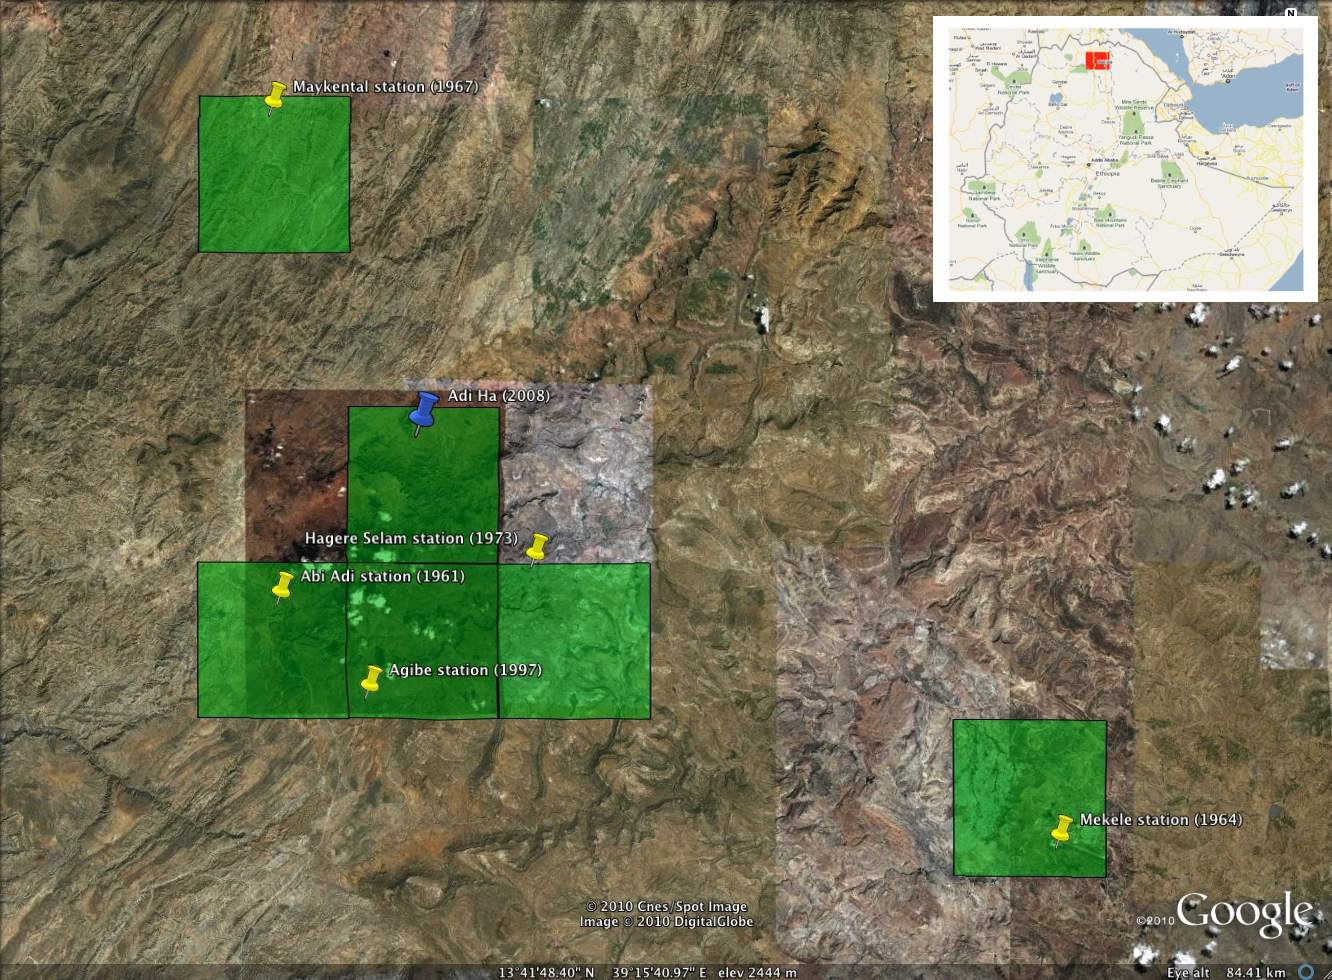
\includegraphics[width=4.5in]{fig_ethiopia_papermap.jpg}
\caption{A map of the 6 locations, where the green squares denote ARC pixels and the pins denote rain station locations. The inset in the upper right corner shows the area of the map with a red rectangular box; this region is in north central Ethiopia.}
\label{fig_ethiopia_map}
\end{center}
\end{figure}

The specifics of the data are as follows:
\begin{itemize}
\item For the first five locations, we have rain station data as well daily measurements from a satellite product called ARC, which is a rainfall proxy based on the temperature of the clouds over an area of about one hundred square kilometers. This comprises $ 5 \times 2 = 10$ time series.
\item For the sixth location, Adi Ha, we have five separate data sources:
\begin{enumerate}
\item One reliable rain station from which we only have 200 days of data from 2009-2010; this is the time series in which we have the most interest, because it is a new, accurate rain station on which we want to base insurance contracts.
\item One unreliable rain station from which we have about 7 years of data from 2000-2009, with about 2 years of missing data interspersed.
\item The ARC satellite proxy.
\item Two additional satellite proxies that are different from ARC.
\end{enumerate}
\end{itemize}

Figure~\ref{fig_overlap} shows the range of observed and missing data for each of these 15 time series; note that the time scale goes back to 1961 for one of the rain stations, but for simplicity, we only consider the time span of 1992-2010 in our model fit, because this span contains most of the data.

\begin{figure}[htbp]
\begin{center}
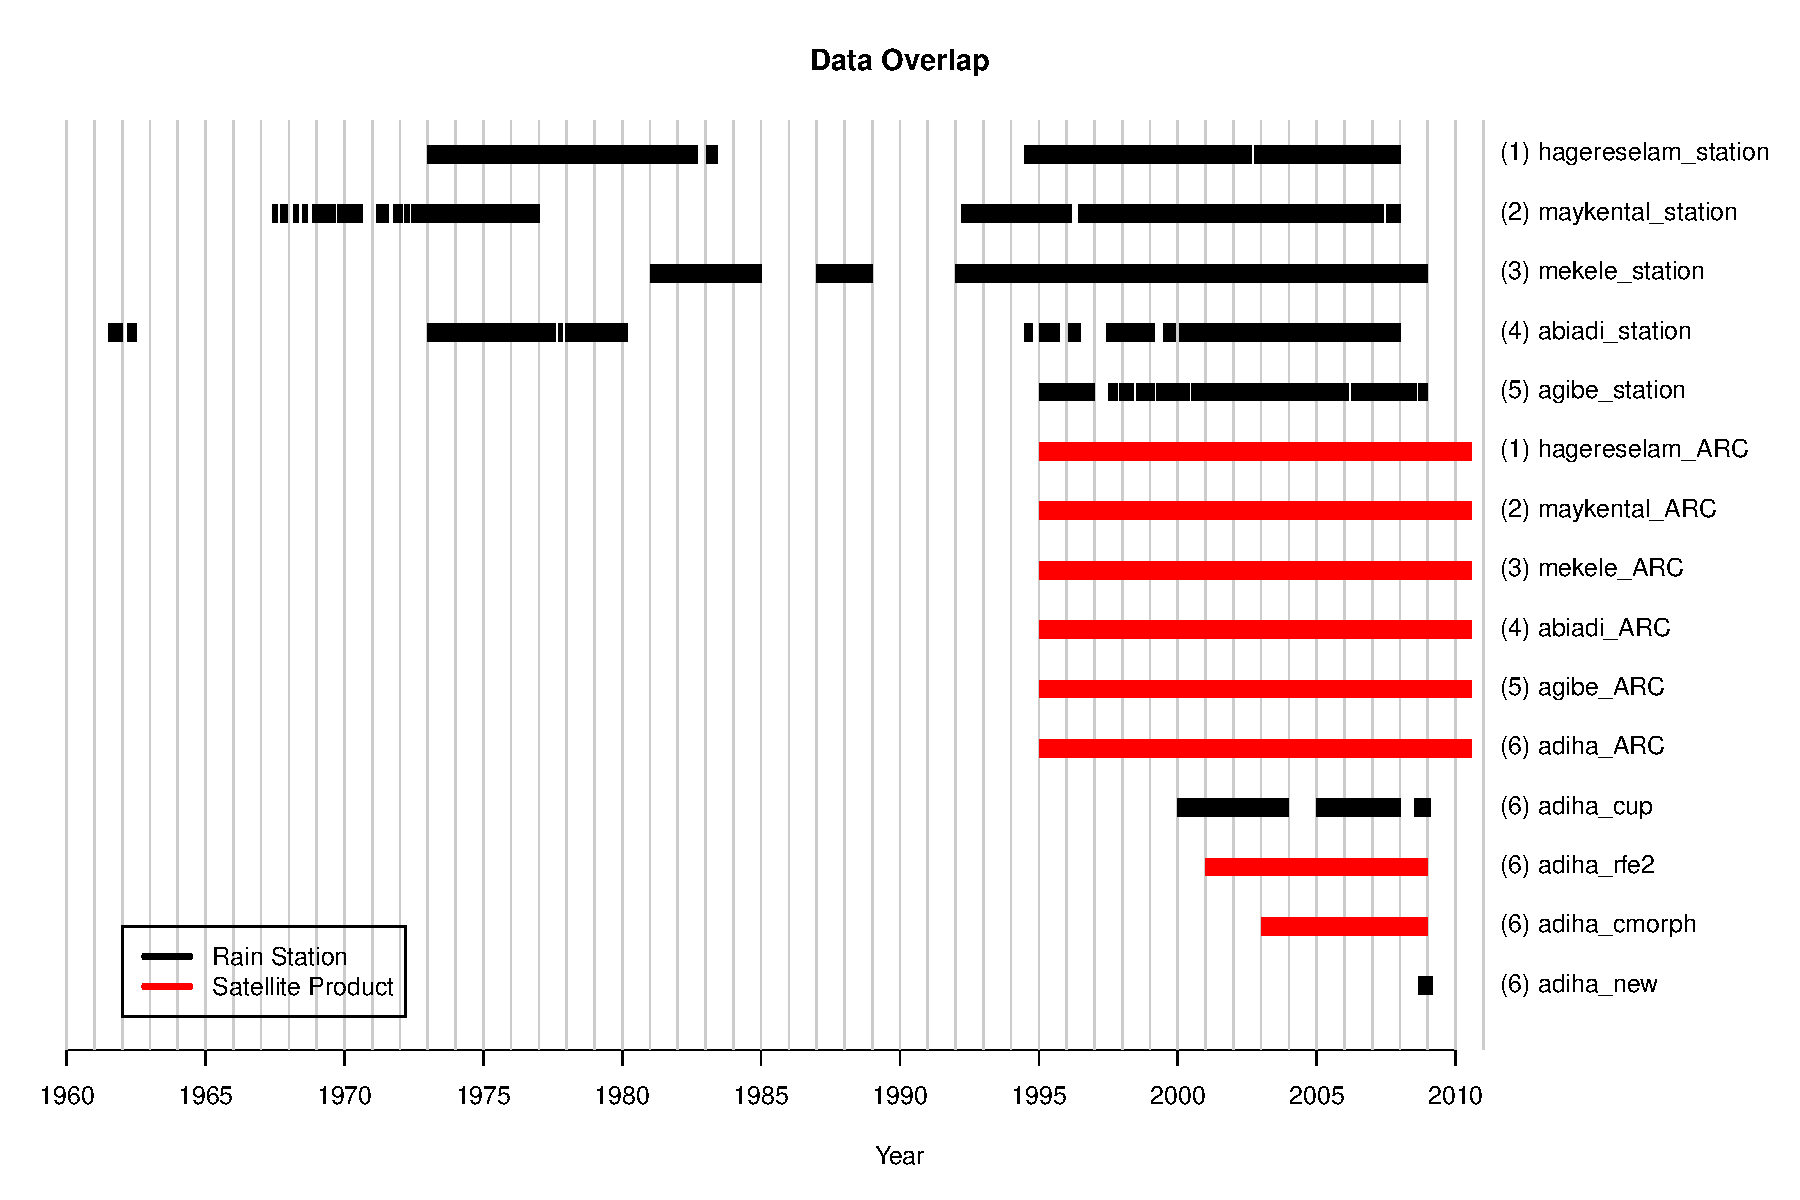
\includegraphics[width=5.0in]{fig_observed_data_new.pdf}
\caption{A visualization of the observed data for each of the 15 time series we model. The black hash marks denote rain station data, and the red hash marks denote satellite-based data.}
\label{fig_overlap}
\end{center}
\end{figure}

Table~\ref{tab_summary} contains some background information and summary statistics related to each time series of daily rainfall. For each time series we record the latitude, longitude, and elevation of the location where measurements were made, and the number of days of observed data. The maximum distance between locations is about 70 kilometers (between Mekele in the southeast and Maykental in the northwest).
\begin{table}[htdp]
\caption{Background information about the 15 time series}
\begin{center}
\begin{tabular}{|l|l|l|l|r|r|}
\hline
 & Site & Latitude & Longitude & Elev. (m) & Num. Obs \\
\hline
1 & Hagere Salaam & $13^\circ$ 38' 49'' & $39^\circ$ 10' 19'' & 2625 & 4887 \\
2 & Hagere Salaam (ARC) & '' & '' & '' & 5632 \\
3 & Maykental & $13^\circ$ 56' 13'' & $38^\circ$ 59' 49'' & 1819 & 5620 \\
4 & Maykental (ARC) & '' & '' & '' & 5632 \\
5 & Mekele & $13^\circ$ 28' 1'' & $39^\circ$ 31' 1'' & 2247 & 6205 \\
6 & Mekele (ARC) & '' & '' & '' & 5632 \\
7 & Abi Adi & $13^\circ$ 37' 19'' & $39^\circ$ 0' 10'' & 1849 & 4205 \\
8 & Abi Adi (ARC) & '' & '' & '' & 5632 \\
9 & Agibe & $13^\circ$ 33' 43'' & $39^\circ$ 3' 43'' & 1952 & 4722 \\
10 & Agibe (ARC) & '' & '' & '' & 5632 \\
11 & Adi Ha (ARC) & $13^\circ$ 43' 48'' & $39^\circ$ 05' 38'' & 1713 & 5632 \\
12 & Adi Ha (Rain Station - Manual) & '' & '' & '' & 2769 \\
13 & Adi Ha (RFE2) & '' & '' & '' & 2920 \\
14 & Adi Ha (CMorph) & '' & '' & '' & 2190 \\
15 & Adi Ha (Rain Station - Automatic) & '' & '' & '' & 186 \\
\hline
\end{tabular}
\end{center}
\label{tab_summary}
\end{table}%

\section{Exploratory Data Analysis}
In this part of Ethiopia, the rainy season lasts roughly from June to October. Figure~\ref{fig_eda} shows the percentage of rainy days and the average amount of rain as a function of the time of year for each time series. The basic modeling strategy will be to use a set of periodic functions to model rainfall as a function of the season of the year.
\begin{figure}[ht]
\begin{center}
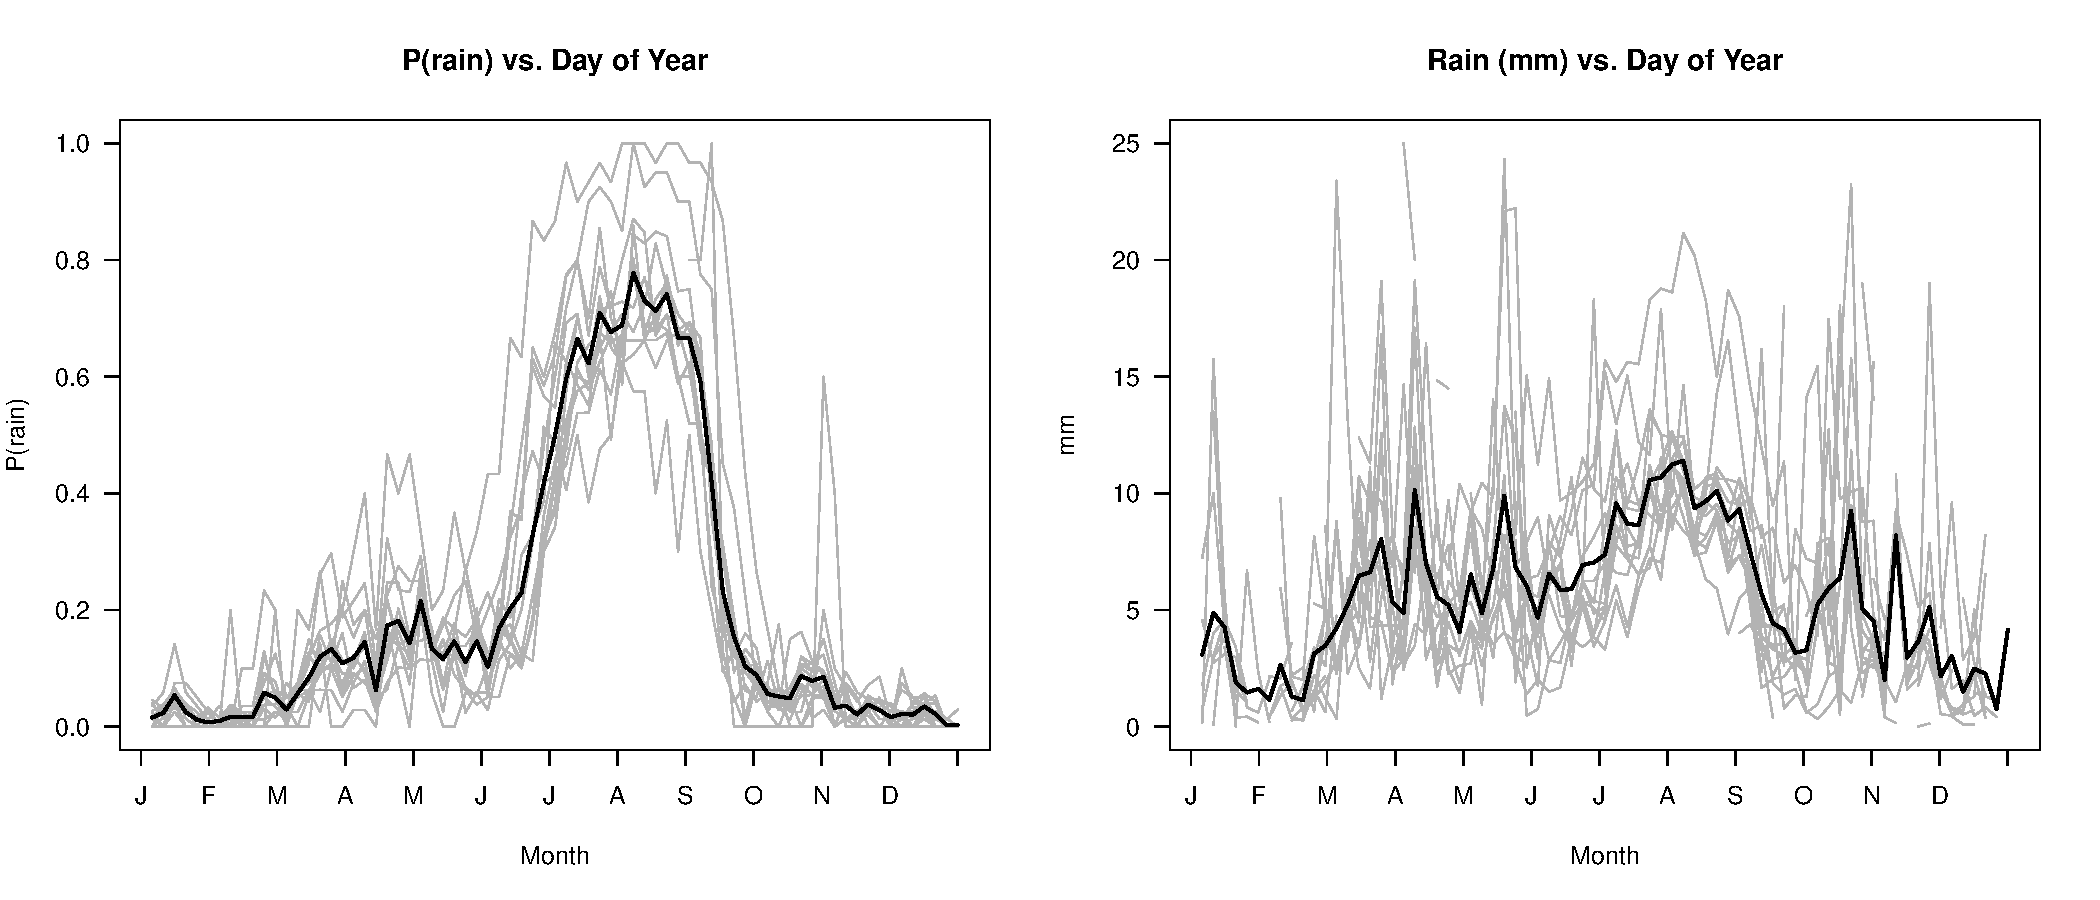
\includegraphics[width=6.5in]{fig_eda.pdf}
\caption{Plots of the percentage of rainy days (pooled into 5-day bins) and the average amount of rain as a function of the season. The gray lines are for each of the 15 individual time series, and the black lines are averaged across all 15 time series.}
\label{fig_eda}
\end{center}
\end{figure}

We are also interested in the difference, on average, between the measurements of rainfall based on the ARC satellite proxy and the rain stations. Comparing rainfall frequencies pooled over 5-day periods, averaging across all parts of the year and all five locations with exactly one rain station and one ARC measurement, we find that the ARC records about 3\% fewer days of rainfall than the rain stations. Across locations, this difference ranges from about -6\% (Hager Selam) to  +1\% (Agibe).



\section{The Model}
Our model consists of two main components: a model for the binary variable of whether or not it rains on a given day (called the frequency model), and a model for the amount of rainfall, given that there was rainfall (called the intensity model). In this paper, we are most interested in the frequency model; the methods we use to model frequency, though, could also be used to model intensity.

Let us first set up some notation. Let $S=6$ denote the number of locations where we measure rainfall, and $\bJ = \{2,2,2,2,2,5\}$ is the vector denoting the number of daily rainfall time series observed for each of the $S$ locations. The total number of days in our time series is $T=6679$ days, from 1/1/1992 through 7/28/2010. Let $V_{stj}$ denote the amount of rainfall, measured in mm, for location $s \in (1,...,S)$, day $t \in (1,...,T)$, and time series $j = (1,...,J_s)$. Let $Y_{stj} = 1(V_{stj}>0)$, an indicator of whether there was non-zero rainfall for site $s$, day $t$, and time series $j$. Last, let $D_{ik}$ denote the Euclidian distance between site $i$ and $k$, for $i,k \in (1,...,S)$.

We model the indicator of nonzero rainfall, $Y_{stj}$, using a hierarchical Bayesian probit regression model, where the levels of the hierarchy correspond to different sources of variation:

\begin{align}
Y_{stj} = 1(Z_{stj} &> 0),\\
Z_{stj} \sim \text{N}&(W_{st} + \alpha_s X^\text{ARC}_{sj}, \tau_s^2),\\
\bW_t &\sim N_S(\bX_t \bbeta, \bR),\\
&\beta_{ps} \sim \text{N}(\mu_p, \sigma^2_p), \hspace{2.04in} \text{for $p \in (1,..,K)$}\\
&\bR=\{r_{ik}\}, r_{ii}=1, r_{ik} = \exp(-\lambda d_{ik}) \hspace{0.7in} \text{for $i,k \in (1,..,S)$}\\
&\bX_t = (1,t,\sin(2\pi t \omega_1), \cos(2\pi t \omega_1),...),\\
\alpha_s &\sim N(\mu_\alpha, \tau^2_\alpha),
\end{align}

where we use relatively flat priors for $\tau$, $\mu_p$, $\sigma_p$, $\lambda$, $\mu_\alpha$, and $\tau_\alpha$.

The explanation of the model is as follows. The first level of the model is a standard probit regression, where we model the observed $Y_{stj}$ as the indicator of whether a normally distributed latent variable denoted $Z_{stj}$ is greater than zero. The next level of the model is essentially a measurement error model: we model $Z_{stj}$ as a normal random variable with a mean centered at $W_{st} + \alpha_s X^\text{ARC}_{sj}$. Here, $W_{st}$ is another latent variable representing whether it \emph{truly} rained at location $s$ on day $t$, and $\alpha_s$ is a bias induced by using the ARC satellite product. $X^\text{ARC}_{sj}$ is an indicator variable of whether time series $j$ at location $s$ is an ARC satellite product. The variance of $Z_{stj}$, $\tau_s$, represents how noisy the observations from multiple sources of data, $j=1,..,J_s$, are for location $s$. For example, we might find that the five Adi Ha time series, each coming from a different source of data (but attempting to measure the true daily rainfall at the same location) are highly variable, whereas the multiple time series from some other location are less variable. We treat the different time series at each location as noisy measurements of the same thing (the ``true" latent variable indicating nonzero rainfall), where the measurement error consists of fixed effects ($\alpha_s$) and random effects (whose variation is modeled by $\tau_s$). This model will also allow us to estimate if the ARC product at each location is sytematically biased to report more or less rainfall than the other sources of data. Note that the ARC bias is modeled as constant across the year, which is an assumption that we could relax in a subsequent model. Also, the errors are homoskedastic ($\tau_s$ does not depend on $t$).

We model the ``true" rainfall latent variables for each site, $W_{st}$, as dependent on each other, via a multivariate normal random variable. The mean of the $S$-length random vector $\bW_t$ is $\bX_t \bbeta$, and the covariance is $\bR$. The covariance matrix depends on only one input, the Euclidean distance between locations, and one unkonwn parameter, $\lambda$. This is how we model the spatial correlation in rainfall between locations (and how it is modeled separately from the noise inherent in the different measurement methods at each location, which is modeled by $\tau_s$). The model assumes that the covariance of pairs of $W_{st}$'s decays exponentially with Euclidian distance at the unknown rate $\lambda$. The mean of $\bW_t$ is related to time, where the cycles per year in $X_t$ are $365 \times \bomega = (1, 2, 3, 1/7)$, which are frequencies chosen based on exploratory data analysis. The term that accounts for a cycle every 7 years is interesting, because such a cycle would roughly correspond to an el Nino event. Note that we also model a linear trend in rainfall frequency for each location via $\beta_{2s}$.

The rest of the model is straightforward. We shrink the $\beta_{ps}$'s for each location toward a common mean $\mu_p$. We also model the ARC biases, $\alpha_s$ as normal random variables with an unknown mean, $\mu_\alpha$, and variance $\tau_\alpha^2$.

\section{Fitting the Model}
We used MCMC to fit the model. There was a combination of gibbs steps and metropolis steps. It took about 60 minutes to sample 3 chains of 2000 iterations each.

\section{Simulation Study}
First, we did a simulation study, where we simulated data from a set of known parameters. These parameter values were chosen to approximate values that could have produced our observed data, based on EDA. The size of the simulated data set was similar to the real data in both dimensions (the number of time series and the number of days).

The results were very encouraging: we were able to precisely estimate the spatial correlation between locations as well as the variability of different data sources within single locations. Figure~\ref{fig_sim_sum1} shows trace plots for $\lambda$, $\mu_\alpha$, and $\tau_\alpha$. All three parameters were well-estimated, and convergence was relatively quick. Furthermore, we were able to accurately estimate different ARC biases, $\alpha_s$ for each location, as well as different amounts of variability at each location, $\tau_s$. Last, the estimates of $\bbeta$ were accurate.
\begin{figure}[htbp]
\begin{center}
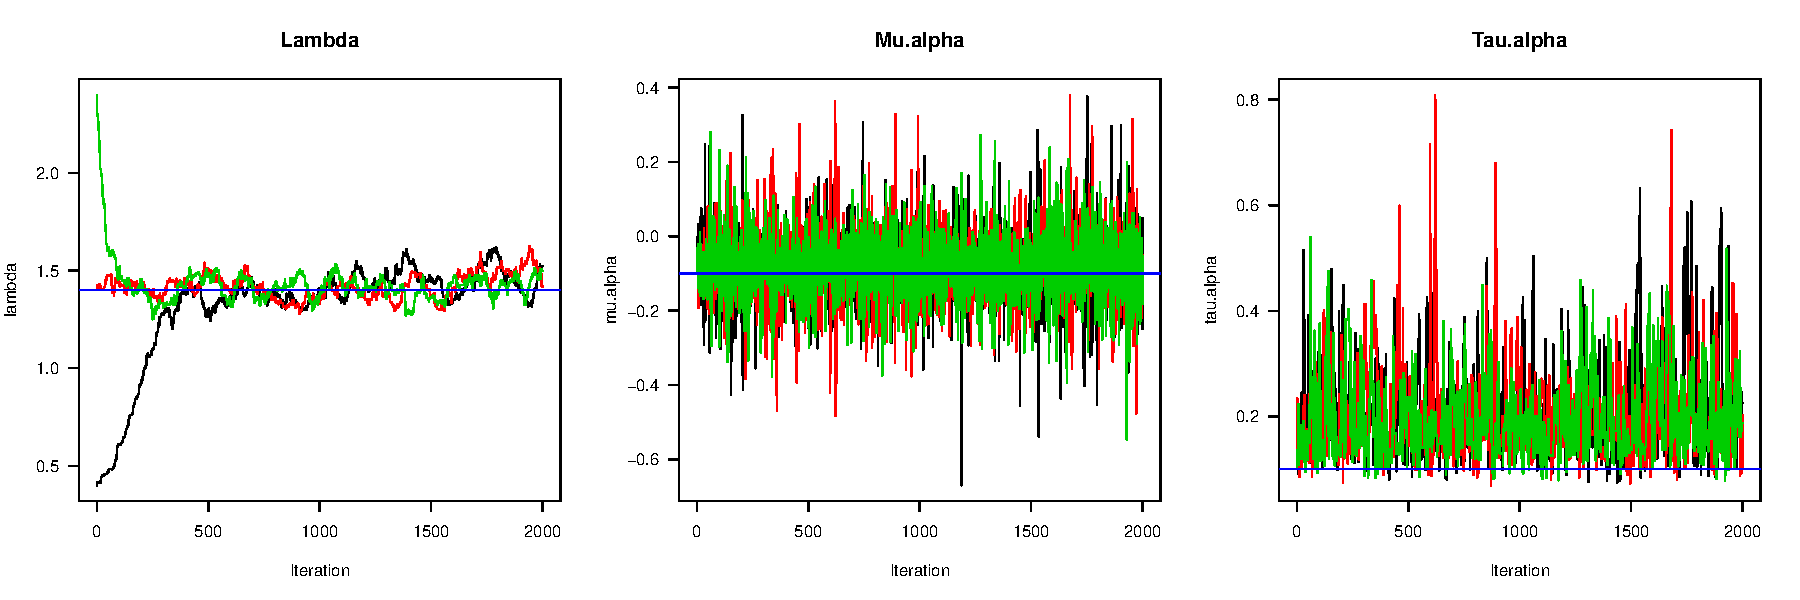
\includegraphics[width=6.0in]{fig_sim_sum1.pdf}
\caption{Simulation study results for $\lambda$, $\mu_\alpha$, and $\tau_\alpha$, where the horizontal blue lines represent the known true values of the parameters.}
\label{fig_sim_sum1}
\end{center}
\end{figure}




\section{Results}
The results on the real data are equally encouraging. We 









\end{document}




\hspace{0.3in} $Y_{stj} = 1(Z_{stj} > 0),$\\
\vspace{0.08in}
\hspace{0.3in} $Z_{stj} \sim N(W_{st} + \alpha_s X^\text{ARC}_{sj}, \tau_s^2),$\\
\vspace{0.08in}
\hspace{0.5in} $\bW_t \sim N_S(\bX_t \bbeta, \bR),$\\
\vspace{0.08in}
\hspace{0.7in} $\beta_{ps} \sim N(\mu_p, \sigma^2_p),$\\
\vspace{0.08in}
\hspace{0.7in} $\bR=\{r_{ik}\}$, $r_{ii}=1$, $r_{ik} = \exp(-\lambda d_{ik}), \hspace{1in} \text{for $i,k \in (1,..,S)$}$\\
\vspace{0.08in}
\hspace{0.7in} $\bX_t = (1,t,\sin(2\pi t \omega_1), \cos(2\pi t \omega_1),...),$\\
\vspace{0.08in}
\hspace{0.5in} $\alpha_s \sim N(\mu_\alpha, \tau^2_\alpha),$\\
\vspace{0.08in}
where we use relatively flat priors for $\tau$, $\mu_p$, $\sigma_p$, $\lambda$, $\mu_\alpha$, and $\tau_\alpha$.


